\appendix{Представление графического материала}

Графический материал, выполненный на отдельных листах,
изображен на рисунках А.1--А.\arabic{числоПлакатов}.
\setcounter{числоПлакатов}{0}

\renewcommand{\thefigure}{А.\arabic{figure}} % шаблон номера для плакатов

\begin{landscape}

\begin{плакат}
    
\includegraphics[width=0.82\linewidth]{posters/p1im.png}
    \заголовок{Сведения о ВКРБ}
    \label{p1im:image}      
\end{плакат}

\begin{плакат}
    
\includegraphics[width=0.82\linewidth]{posters/p2im.png}
    \заголовок{Цели и задачи разработки}
    \label{p2im:image}      
\end{плакат}

\begin{плакат}
    
\includegraphics[width=0.82\linewidth]{posters/p3im.png}
    \заголовок{Концептуальная модель распределенной поисковой системы}
    \label{p3im:image}      
\end{плакат}

\begin{плакат}
    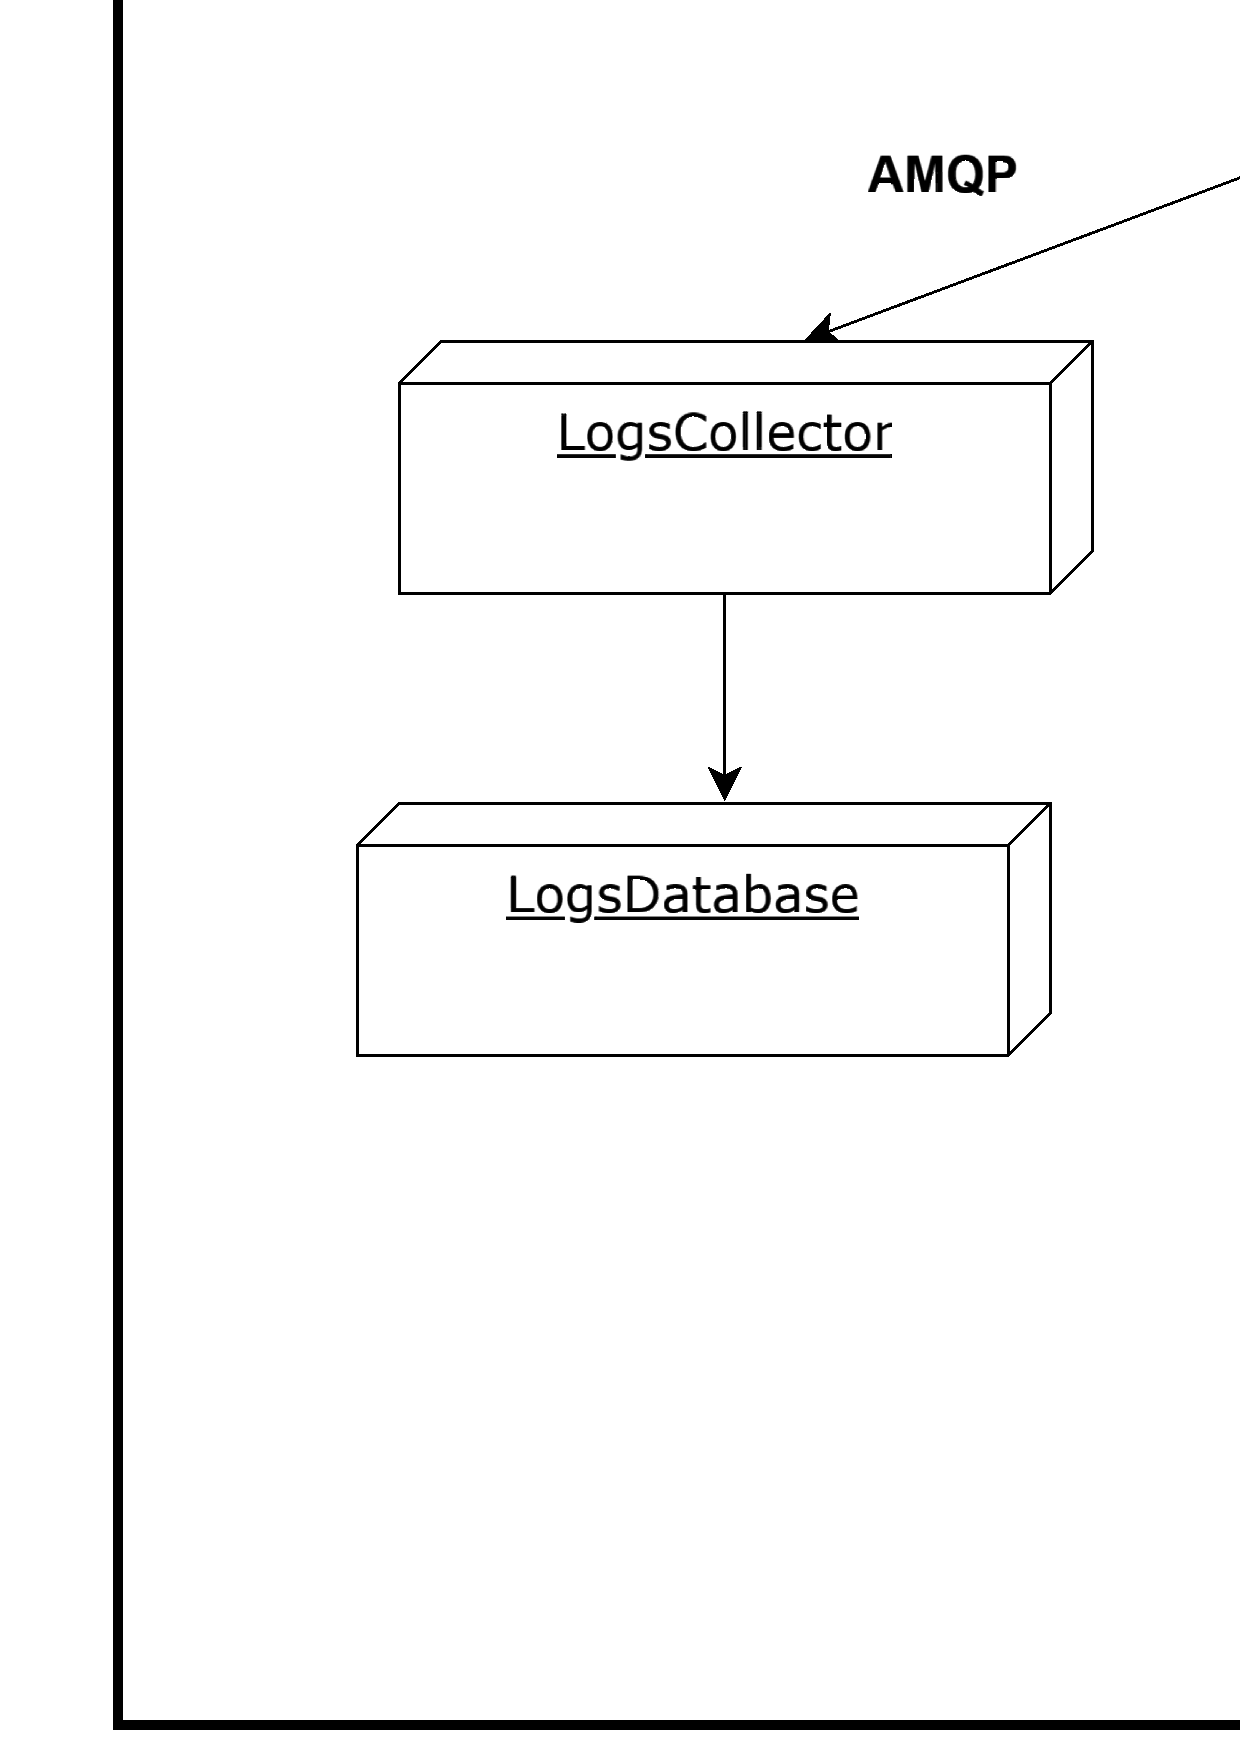
\includegraphics[width=0.82\linewidth]{posters/p4im.png}
    \заголовок{Диаграмма развертывания}
    \label{p4im:image}      
\end{плакат}

\begin{плакат}
    
\includegraphics[width=0.82\linewidth]{posters/p5im.png}
    \заголовок{Диаграмма прецедентов}
    \label{p5im:image}      
\end{плакат}

\begin{плакат}
    
\includegraphics[width=0.82\linewidth]{posters/p6im.png}
    \заголовок{Заключение}
    \label{p6im:image}      
\end{плакат}

\end{landscape}